\chapter{Guía de Uso.}\label{sec:GuiaDeUso}

\paragraph{}En este capítulo se van a explicar las principales funciones del entorno de
desarrollo, así como las principales opciones de cada herramienta provista a los
desarrolladores.

\section{Consideraciones previas}

\paragraph{}Todos los pasos de todas las guías de este capítulo podrán ser seguidas si
previamente se han seguido las indicaciones del cápitulo \ref{sec:ManualDeInstalacion}.

\paragraph{}Al igual que en el capítulo anterior \ref{sec:ManualDeInstalacion}, la guía
de uso estará dividida en: entorno de desarrollo Flutter y entorno de desarrollo Yocto.
Esta separación lógica, tiene sentillo ya que ambas partes pueden funcionar tanto por
separado como juntas. Y ambas partes pueden ser utilizadas para propositos distintos
que el de funcionar juntas.

\section{Entorno de desarrollo Flutter}

\paragraph{}Una vez instalado, el uso del entorno Flutter no deja de ser indéntico a
cómo se usa habitualmente Visual Studio Code para el desarrollo de Flutter. Por ello,
si no se está acostumbrado al desarrollo de Flutter en Visual Studio Code, existen
multitud de guías en internet que lo explican, como la se puede encontrar en el
siguiente enlace:

\paragraph{}\href{https://esflutter.dev/docs/development/tools/vs-code}
{Guía oficial de desarrollo de Flutter en Vscode}

\subsection{Características Principales}

\begin{itemize}
    \item Compatibilidad con la mayoría de sistemas operativos.
    \item Facilidad de instalación.
    \item Fácil de gestionar remotamente.
    \item \gls{IaaC}.
\end{itemize}

\paragraph{}Las principales particularidades de este entorno de desarrollo son las
maneras de inicializar las herramientas para empezar a trabajar. Dicha manera, dependerá
del método de instalación elegido.

\paragraph{}Para empezar a trabajar con el método \emph{desarrollo en container de docker},
cada vez que se abra Vscode habrá que reabrir el proyecto pulsando en el botón del mensaje
emergente que nos aparece al abrir la carpeta de trabajo.

\begin{figure}[H]
    \centering
    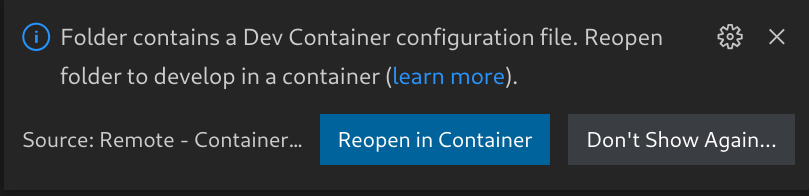
\includegraphics[width=0.75\textwidth]{imgs/dev-container}
    \caption[Mensaje emergente en Vscode]{Mensaje emergente en Vscode.}
    \label{imgs:vscode-devcontainer-2}
\end{figure}

\paragraph{}En caso de que se haya optado por trabajar desde el entorno \emph{Dockerizado}
sólo habrá posibilidad de realizar las siguientes acciones: compilar, ejecutar la aplicación,
lanzar los test y depurar con las opciones del servidor de depueración a través del navegador.
Todas estas acciones salvo la última se realizan por línea de comandos. La depuración,
será limitada y para acceder a ella, debemos abrir en el navegador la IP indicada.

\begin{figure}[H]
    \centering
    \fbox{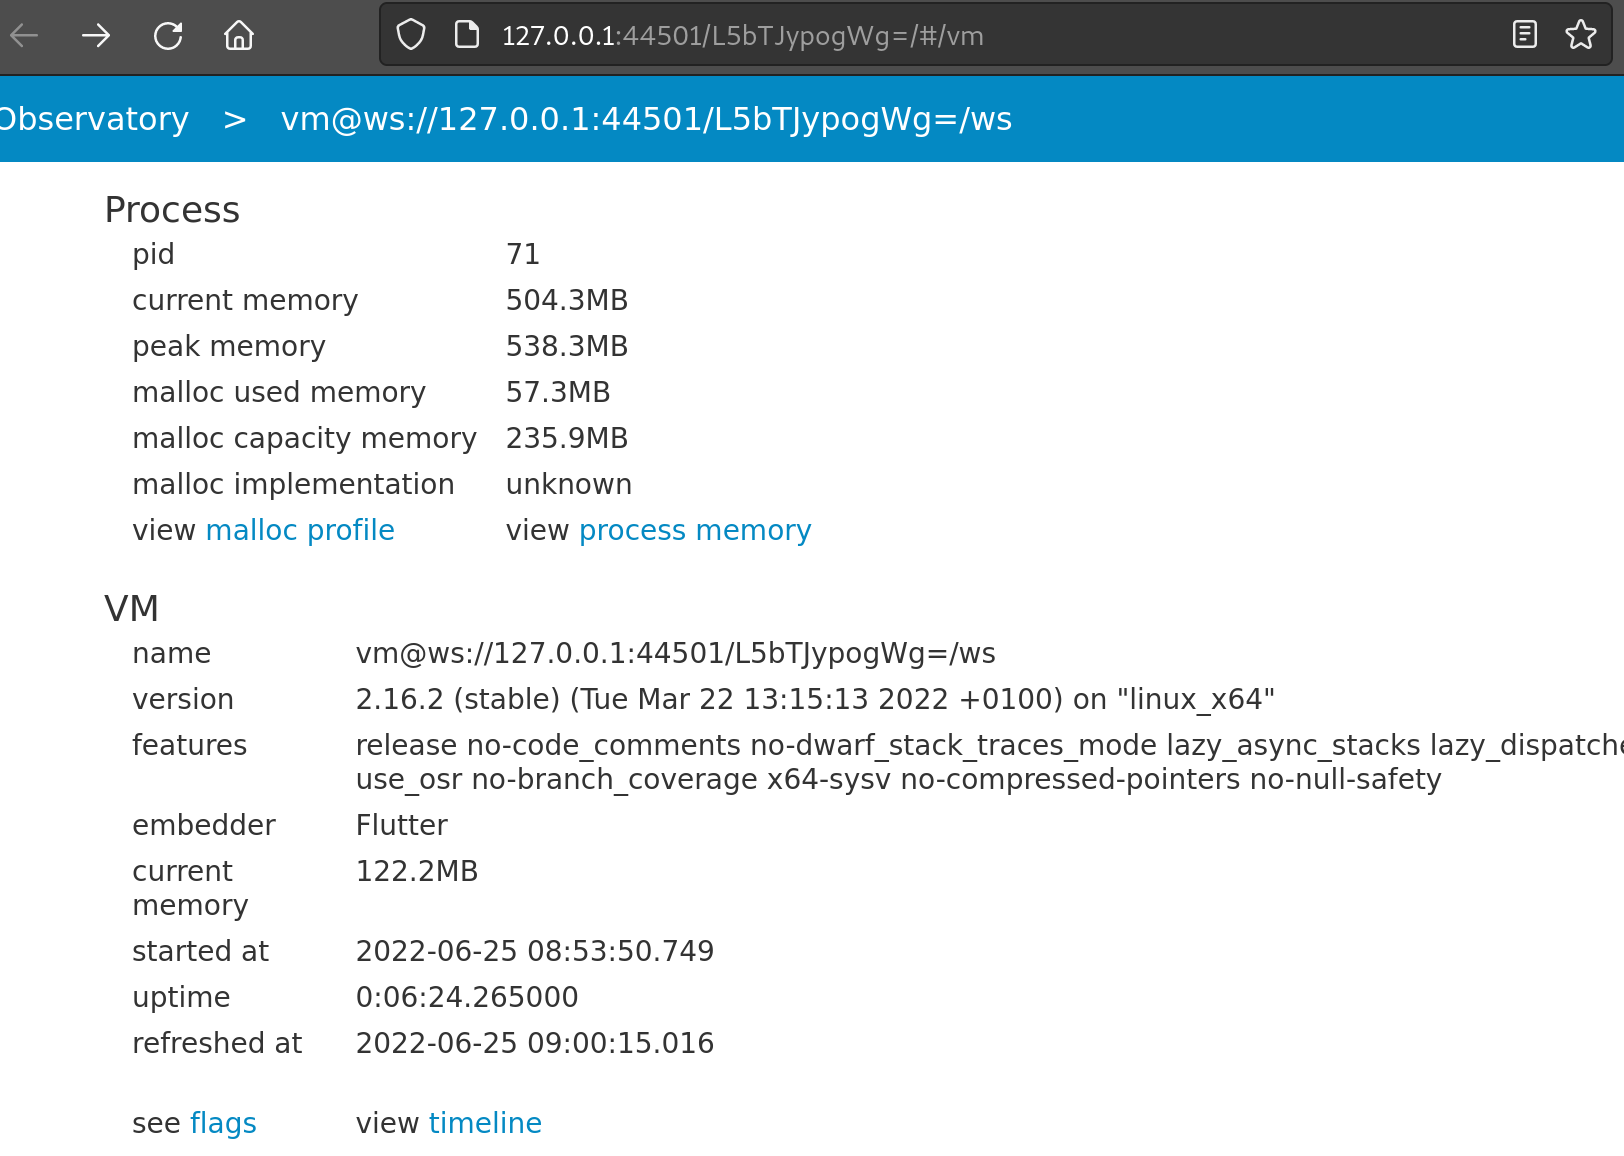
\includegraphics[width=0.75\textwidth]{imgs/devtools}}
    \caption[Navegador con devtools]{Navegador con devtools.}
    \label{imgs:devtools}
\end{figure}

\paragraph{}Si estamos utilizando el entorno en Windows con \gls{WSL2}, entonces una
vez arrancado el entorno \gls{WSL2} debemos arrancar un cliente de escritorio remoto
para visualizar la aplicación.

\begin{figure}[H]
    \centering
    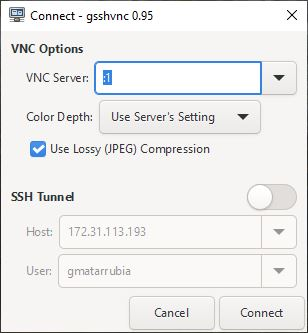
\includegraphics[width=0.40\textwidth]{imgs/gsshvnc-open}
    \caption[Abriendo el cliente gsshvnc]{Abriendo el cliente gsshvnc.}
    \label{imgs:open-gsshvnc}
\end{figure}

\begin{figure}[H]
    \centering
    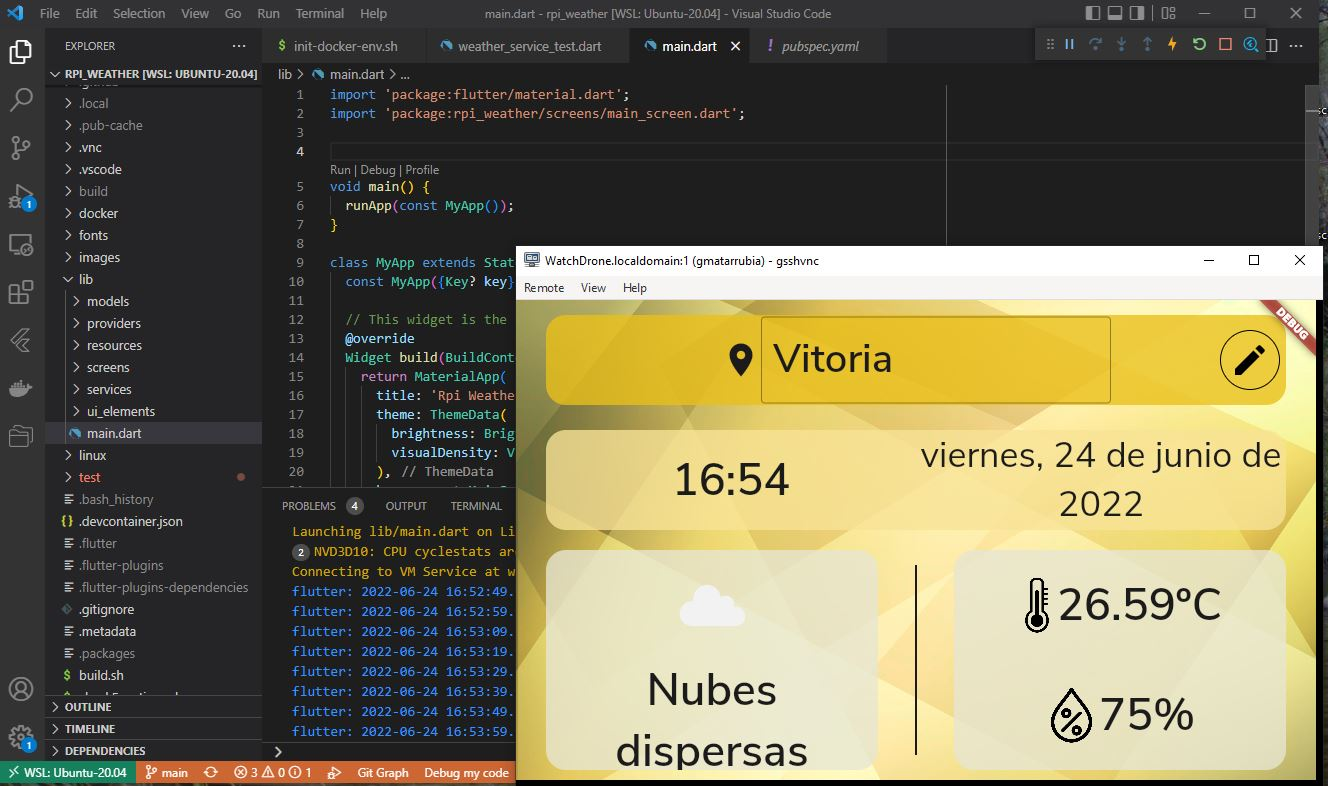
\includegraphics[width=0.90\textwidth]{imgs/wsl2-running}
    \caption[WSL2 + gsshvnc.c]{WSL2 + gsshvnc.}
    \label{imgs:running-gsshvnc}
\end{figure}

\paragraph{}A continuación se muestran las acciones provistas por el entorno de desarrollo.

\subsection{Build}

\paragraph{}Para compilar la aplicación se puede utilizar el siguiente comando por
terminal:

\begin{lstlisting}[style=consola, numbers=left]
    # Usage of ./build.sh [--debug] | [--test]
    $ ./build.sh
\end{lstlisting}

\paragraph{}Como podemos observar, el comando acepta los argumentos: \emph{debug} y
\emph{test}. Por defecto, la aplicación se compila en \gls{release}, salvo que pasemos
el argumento de \emph{debug}. El argumento \emph{test}, se utilizará para compilar y
ejecutar los test. Este argumento invalida al anterior.

\subsection{Ejecutar la app}

\paragraph{}Este comando nos permite ejecutar la aplicación desde una terminal.

\begin{lstlisting}[style=consola, numbers=left]
    # Usage of ./runApp.sh [--debug] | [--release]
    $ ./runApp.sh
\end{lstlisting}

\paragraph{}Los argumentos que admite este comando son: \gls{debug} y \gls{release}.
Qué se corresponden con los modos de ejecución de la aplicación. En caso de querer
ejecutar la y que ésta no haya sido compilada previamente se compilará con el modo
correspondiente antes de ser ejecuta. Por defecto, la app se ejecuta en modo \gls{release}.

\subsection{Limpiar repo}

\paragraph{}Con este comando limpiaremos todos los archivos que habían sido generados
automáticamente.

\begin{lstlisting}[style=consola, numbers=left]
    $ ./cleanAll.sh
\end{lstlisting}

%%%%%%%%%%%%%%%%%%%%%%%%%%%%%%%%%%%%%%%%%%%%%%%%%%%%%%%%%%%%%%%%%%%%%%%%%%%%%%%%%%%%%%

\section{Entorno de desarrollo Yocto}

\paragraph{}Este es el entorno de desarrollo de la distribución FlutterPI. Una distribución
con el kernel de linux para Raspberry Pi basada en poky (yocto) la cuál está pensada
para correr aplicaciones de Flutter. Esto es muy útil para múltiples aplicaciones como
por ejemplo: Máquinas de vending, paneles de información, y muchísimos otros tipos de
HMIs. Este entorno de desarrollo te permite tomarlo de plantilla y desarrollar rápidamente
un sistema HMI, fiable, replicable y altamente personalizable.

\subsection{Características principales}

\paragraph{}Este entorno ha sido diseñado teniendo en cuanta los siguiente aspectos:

\begin{itemize}
    \item Compatibilidad con la mayoría de sistemas operativos.
    \item Facilidad de uso.
    \item Entendible y bien documentado.
    \item Fácil de gestionar remotamente.
    \item Flexibilidad y multipropósito.
    \item \gls{IaaC}.
\end{itemize}

\paragraph{Nota:} Este entorno corre nativamente en sistemas con distribuciones Ubuntu 20.04.
Para el resto de sistemas utilizar cualquiera de los métodos alternativos:

\begin{itemize}
    \item Entorno dockerizado.
    \item Máquina virtual con Ubuntu 20.04.
    \item Entorno en WSL2 (sólo para sistemas Windows 10/11.)
\end{itemize}

\paragraph{}Acudir al capítulo \hyperref[sec:ManualDeInstalacion]{Manual de instalación}
\ref{sec:ManualDeInstalacion} antes de intentar los procedimientos descritos en este
capítulo.

\subsection{Build}

\paragraph{}Para lanzar la generación de la imagen completa con las configuraciones por
defecto utilizar el siguiente comando. El resultado será una imagen arrancable en una
Raspberry Pi el cuál arrancará una aplicación Flutter al comienzo.

\begin{lstlisting}[style=consola, numbers=left]
    $ ./build.sh
\end{lstlisting}

\paragraph{}Antes de empezar la generación, el entorno te preguntará la configuración
Wi-Fi para conectarse a un punto de acceso (ssid + pass). Ésto se puede saltar si
previamente se han configurado las variables de entorno: \emph{WIFISSID} y \emph{WIFIPASS}.

\paragraph{}Para más información sobre los aspectos del script de build pueden ser
consultados con el comando:

\begin{lstlisting}[style=consola, numbers=left]
    $ ./build.sh --help
    This script help you with the initial configuration and with the build process.
    you can use this script with these options:

    -v | --verbose) Prints more detailled output.

    -bc | --bitbake-cmd) Performs your custom bitbake/devtool command.

    --shell) Opens a bitbake shell without do anything else.

    -wi | --wifi-interactive) For setting Wi-Fi settings.

    -d | --debug) Enables debug features on the local.conf

    -h | --help) Prints this useful help :)
\end{lstlisting}

\subsection{Comando de build personalizados}

\paragraph{}Mediante los argumentos -bc <"custom command"> o --bc <"custom command">,
se puede pasar un comando personalizado al entorno de Yocto. Ésto es especialmente útil
para pasar comandos como: bitbake, bitbake-getvar o devtool por citar unos pocos. Para
hacerse una mejor idea de los usos que puede tener, se presentan unos ejemplos:

\begin{lstlisting}[style=consola, numbers=left]
    # Comando para ver las versiones de todas las recipes de flutter
    $ ./build.sh --bitbake-cmd "bitbake -s | grep flutter"

    # Comando para hacer "clean" de la compilacion de una recipe especifica
    $ ./build.sh -bc "bitbake -D wifi -c clean"

    # Comando para ver las capas analizadas y su preferencia
    $ ./build.sh --bitbake-cmd "bitbake-layers show-layers"
\end{lstlisting}

\subsection{Lanzar el modo Sesión Interactiva}

\paragraph{}Esta es una manera potente de depurar y desarrollar tus recipes o tus
aplicaciones flutter. Ya que abres una terminal en la que puedes lanzar comandos como
los anteriores de manera interactiva e iterativa. También da acceso a usar el \gls{eSDK}.

\begin{lstlisting}[style=consola, numbers=left]
    $ ./build.sh --shell
\end{lstlisting}

\paragraph{}Algunos ejemplos de comandos que puedes utilizar dentro de la terminal interactiva:

\begin{itemize}
    \item bitbake
    \item bitbake-getvar
    \item bitbake-layers
    \item devtool
\end{itemize}

\subsection{Limpieza}

\paragraph{}Se proveé del siguiente comando para borrar la mayoría de los archivos generados
automáticamente.

\begin{lstlisting}[style=consola, numbers=left]
    $ ./cleanAll.sh
    # Para una limpieza total usar el siguiente comando.
    # Usar con precaucion ya que se pederan todos los cambios no guardados en git.
    $ git clean -fdx
\end{lstlisting}


%las referencias a artículos se ponen con \cite,
%las referencias a glosario \gls,
%y las referencias a ecuaciones \eqref
%las referencias a imgenes, tablas o figuras o secciones
% se ponen con \ref (sólo número) o con \hyperref[sec:X]{text}
